\section{Thursday, February 9th}
\subsection{Galileo AI}
``Galileo AI creates delightful, editable UI designs from a simple text description. It empowers you to design faster than ever.''

\subsection{Review: Modes}
Last time we went over the Caps Lock key and how it was an example of a mode.

We also talked about quasimodes -- the discomfort of having to hold the Shift button down reminds you that you are still in the \textit{uppercase editing} mode.

\begin{important}
If you forget which mode you are in, you will have the source of numerous errors.
\end{important}

\subsubsection{Keyboard Modes: QWERTY, QWERTZ, AZERTY}
When typing in English vs German, the same buttons can map to letters and muscle memory can work against the User.

\subsubsection{Air France Flight 447}
In 2009, the plane switched modes due to a broken sensor, without alerting the Pilots. Then when the pilots tried to change the direction, they went into Gimbal Lock, from which they could not recover.

\subsection{Modeling Human Performance}
\subsubsection{Motivation}
This is useful to 
\begin{itemize}
    \item react to situations which we did not see -- broader applicability.
    \item A general solution by falling back on stuff we have seen before.
    \item Finally, we don't have to have observe things difficulty but we can extrapolate to unseen criteria
\end{itemize}
You can also react to designs without actually building them.

\begin{important}
Note that even today we still don't have a perfectly comprehensive model -- we must still fallback upon the \textbf{design cycle}.
\end{important}

\subsubsection{Model Information Processor Theory}
This makes the assumption that humans take in data from a bunch of sensors (embedded systems) that go through a perceptual processor and the brain is just a distributed system consisting of multiple computers.
\begin{shaded}
Note that this is probably inaccurate but it predicts performance well.
\end{shaded}

\myparagraph{Perceptual Processor}
We take in features that are visual, audio, haptic, etc.

Our attention is selective and is very fast in dropping details. This is done via pre-attentive features (stuff that pop out at you) such as color (most prominently), shapes, curvature, size, convexity, and many more.
\begin{important}
Note that these cannot be combined -- pre-attentive features only work in isolation -- conjunctions do not work.
\end{important}

\begin{shaded}
Note that the perceptual processor has a cycle time for quantum experience of 100ms.

This is similar to what we see in CS61C w.r.t. how much can be processed, stuff faster cannot be processed.
\end{shaded}

\submyparagraph{Michotte Demonstration}
Causality falls off a cliff between 80 and 100 ms and after that, events are seen as indpendent.

\myparagraph{Memory}
Humans usually repack information as letters or numbers (abstract embeddings with meaning assigned to them) instead of series of pixels with brightness values.

\submyparagraph{Attention Span}
Humans can usually only remember at most $7\pm2$ things at once.

\begin{shaded}
    Attention Span: Interruptions > decay time.
\end{shaded}

The more things you are remembering, the longer the access time it will take to remember it will be.

This is analogous to how a CPU only has a limited number of registers for short-term memory.

\submyparagraph{Long-Term Memory}
In contrast to Short-Term attention span (STM), we also have a longer to access yet bigger Long-Term Memory (LTM).

\begin{shaded}
    There is no known limit for the capacity of Human's Long Term Memory.

    But it is hard to make sure the semantic encoding goes to LTM and not STM. Remembering/retrieving information is also an issue of concern.
\end{shaded}

\myparagraph{Cognitive Processor}
Humans are fundamentally not a multi-core machine -- you can only focus on one thing at a time -- you work in serial (multi-tasking is really just low-latency multiplexing).

\submyparagraph{Flight Eastern 401}
In 1972, the aircraft crashed due to the crew focusing on a `landing gear' indicator which overrode the `crash imminent' indicator to their senses, and made them miss the fact a crash ws imminent

\submyparagraph{Stroop Effect}
The meaning and visual infromation streams conflict and thus confuse your cognitive processor leading to higher latency.

\submyparagraph{Input Stratification}
You can calculate the net latency via adding each cognitive cycle for each processor (visual -- for reading, processing -- for classifying, motor -- for pushing a button, etc).

\begin{important}
    However this does not work since this is not accurate for complex tasks.
\end{important}

Different tasks have different difficulties. Use pre-attentive features or slow-motion to prolong videos if you want the User to see causality in something that occurs very fast.

\subsubsection{Stage Theory}
\myparagraph{Recognition over Recall}
Design for recognition %(given options) 
over recall (info reproduced from memory).

You have probably heard of Snow White \& the Seven Dwarfs but if you are asked to recall the names of the 7 Dwarfs it will probably be non-trivial to do so.

However if I give you a word bank and ask you to choose which are the names, then the task becomes much easier.

\subsection{Decision Making and Learning}
\subsubsection{Hick's Law: Decision Paralysis}
The time cost of taking a decision, $T$, depends on the number of options $n$:
\begin{equation}
    T = a + b\log_2(n+1)
\end{equation}
where $a, b$ are empirically derived constants. $a = \min$ time it takes to do the task (y-intercept), and $b$ = what human muscle group is being used and how quick that works.

This is why supermarkets make it hard to find products, as well as why they display so many products -- to overload your brain into thinking you need more than what you came for.

\subsubsection{Power Law of Practice}
Task time on the $n^{\text{th}}$ trial follows a power law:
\begin{equation}
    T_n = T_1 n^{-a} + c
\end{equation}
\begin{shaded}
    Main Idea: \textbf{You get faster the more times you do something.}
\end{shaded}
This means that it will take longer for visitors who are unfamiliar versus experts with the given technology. This also makes it hard to switch to new, unfamiliar, technologies as your muscle memory has already been built.

\subsection{Pointing}
\subsubsection{Fitts' Law: Distance and Target Size}
This is a foundational Model for any UI designer to know about.

\begin{equation}
    T = a + b\log_2(D/S+1)
\end{equation}
where $D$ = distance, and $S$ = size (and $[a, b] = $ [start/stop time, speed] are empirically derived constants).

\myparagraph{Index of Difficulty}
We can also formulate the Index of Difficulty:
\begin{equation}
    \text{ID} = \log_2(D/S + 1)
\end{equation}
This tells us that $T\uparrow$ as $D\uparrow$ \\
and that $T\downarrow$ as $S\uparrow$.

\begin{shaded}
    If we have a bigger button then it should be easier and faster to click on. This is a due to $S\uparrow$.
\end{shaded}

\myparagraph{Fitts' Law Tasks}
On a touchscreen, tapping and dragging are fundamental Fitts' Law Tasks.

On your laptop, Fitts' Law Tasks are moving your mouse pointer and clicking.

\subsubsection{The Power of Right-clicking: having options come to you}
Instead of having to drag your cursor across the screen, it is more optimal if you can have the list of options come to you. When you right click, a bar of options appears, this exploits Fitt's Law by making $D\to0$.


\subsection{Bandwidth of Human Muscle Groups}
\begin{center}
    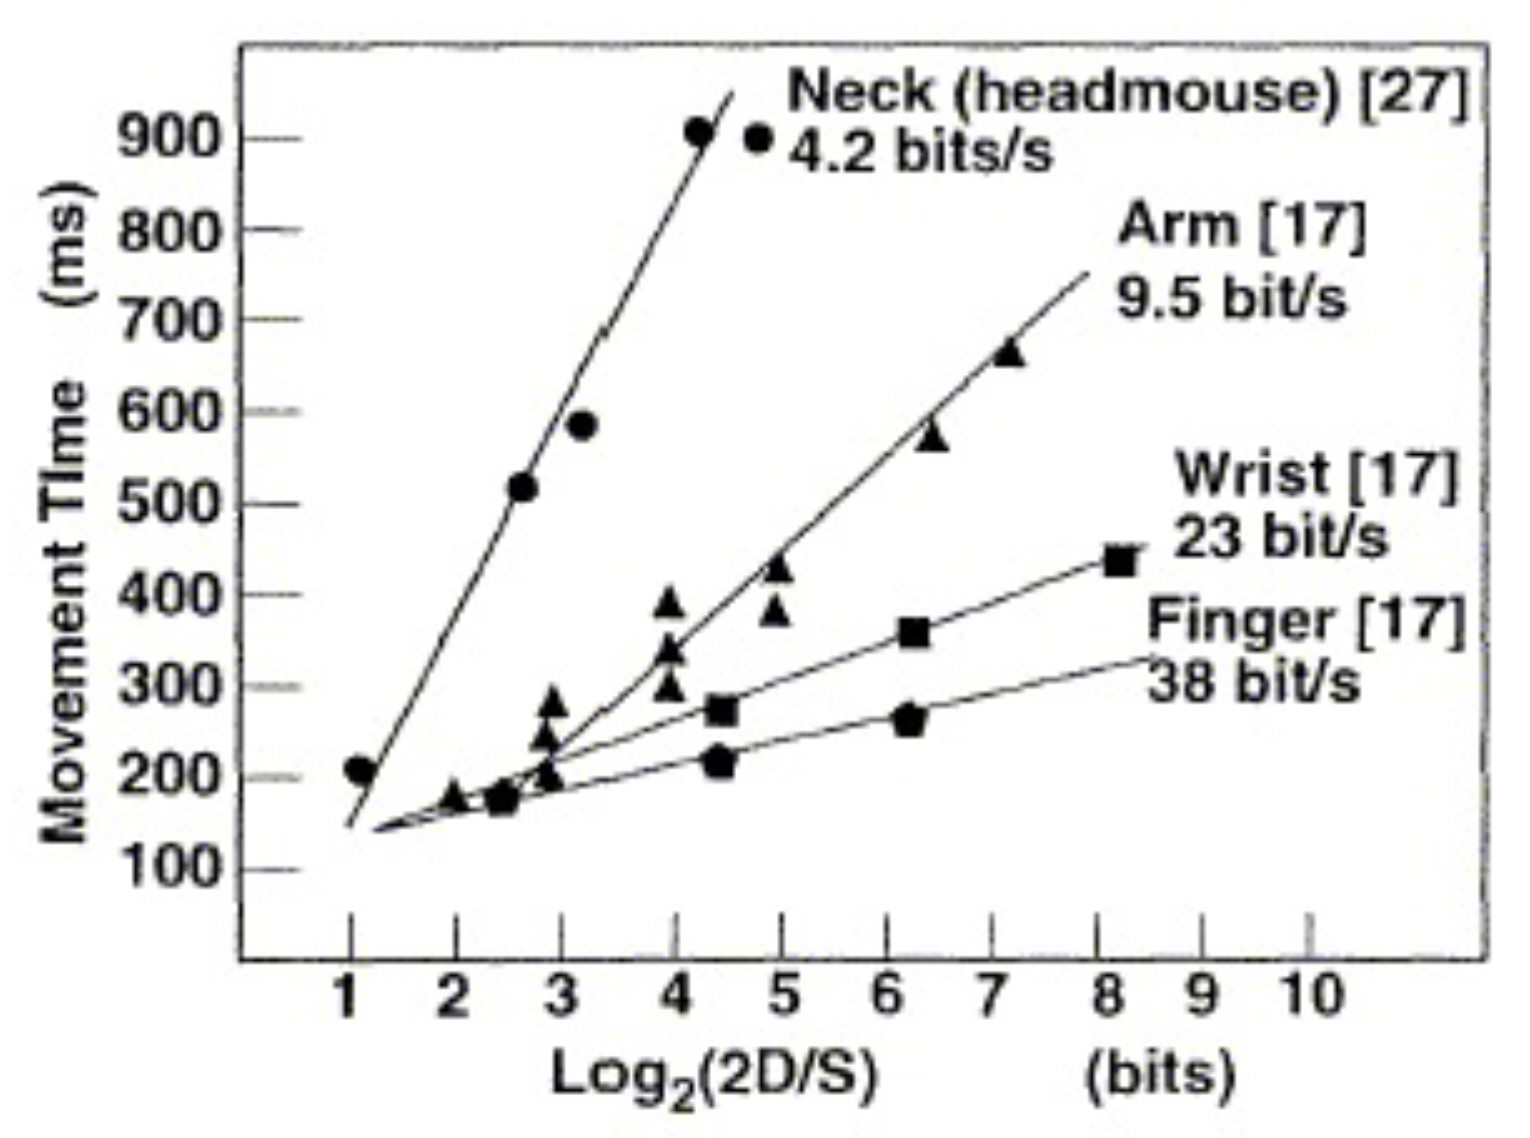
\includegraphics[scale=0.23]{lectures/wk4/img/bandwidth.png}
\end{center}
VR headsets are non-optimal as using fingers instead of neck to click on menus/swipe/move is a \>10x speedup.
